\section{Case Study: EBR-II Liquid Metal Fire Scenario}
\label{sec:case_study_ebr2}
We apply the proposed optimization method to an event tree from the Experimental Breeder Reactor-II (EBR-II) Level I PRA \citep{chang_experimental_2018}. The potential initiating event is a leak in the piping loop of the reactor's shutdown cooler, which uses sodium-potassium (NaK) coolant. Air intrusion near NaK can cause fire hazards. The event tree, shown in Figure \ref{fig:ebr2_sdfr_et} enumerates whether (i)~the liquid-metal fire is detected in time (\(\text{LMFD}\)), (ii)~a reactor scram is successfully initiated (\(\text{RFIR}\)), (iii)~the fire is classified as severe or limited (\(\text{LLRF}\)), (iv)~a plant-level fire suppression system fails or succeeds (\(\text{SSSD}\)), and (v)~critical secondary systems remain operational (\(\text{SYSO}\)). These conditional events interact to form multiple end-states, labeled \(\text{SDFR-0}\) through \(\text{SDFR-8}\). Some end-states represent minimal impact (e.g., immediate fire detection and promptly executed scram), whereas others lead to more severe conditions (e.g., no detection and system failures yielding potential core damage).

\begin{figure}[h]
  \centering
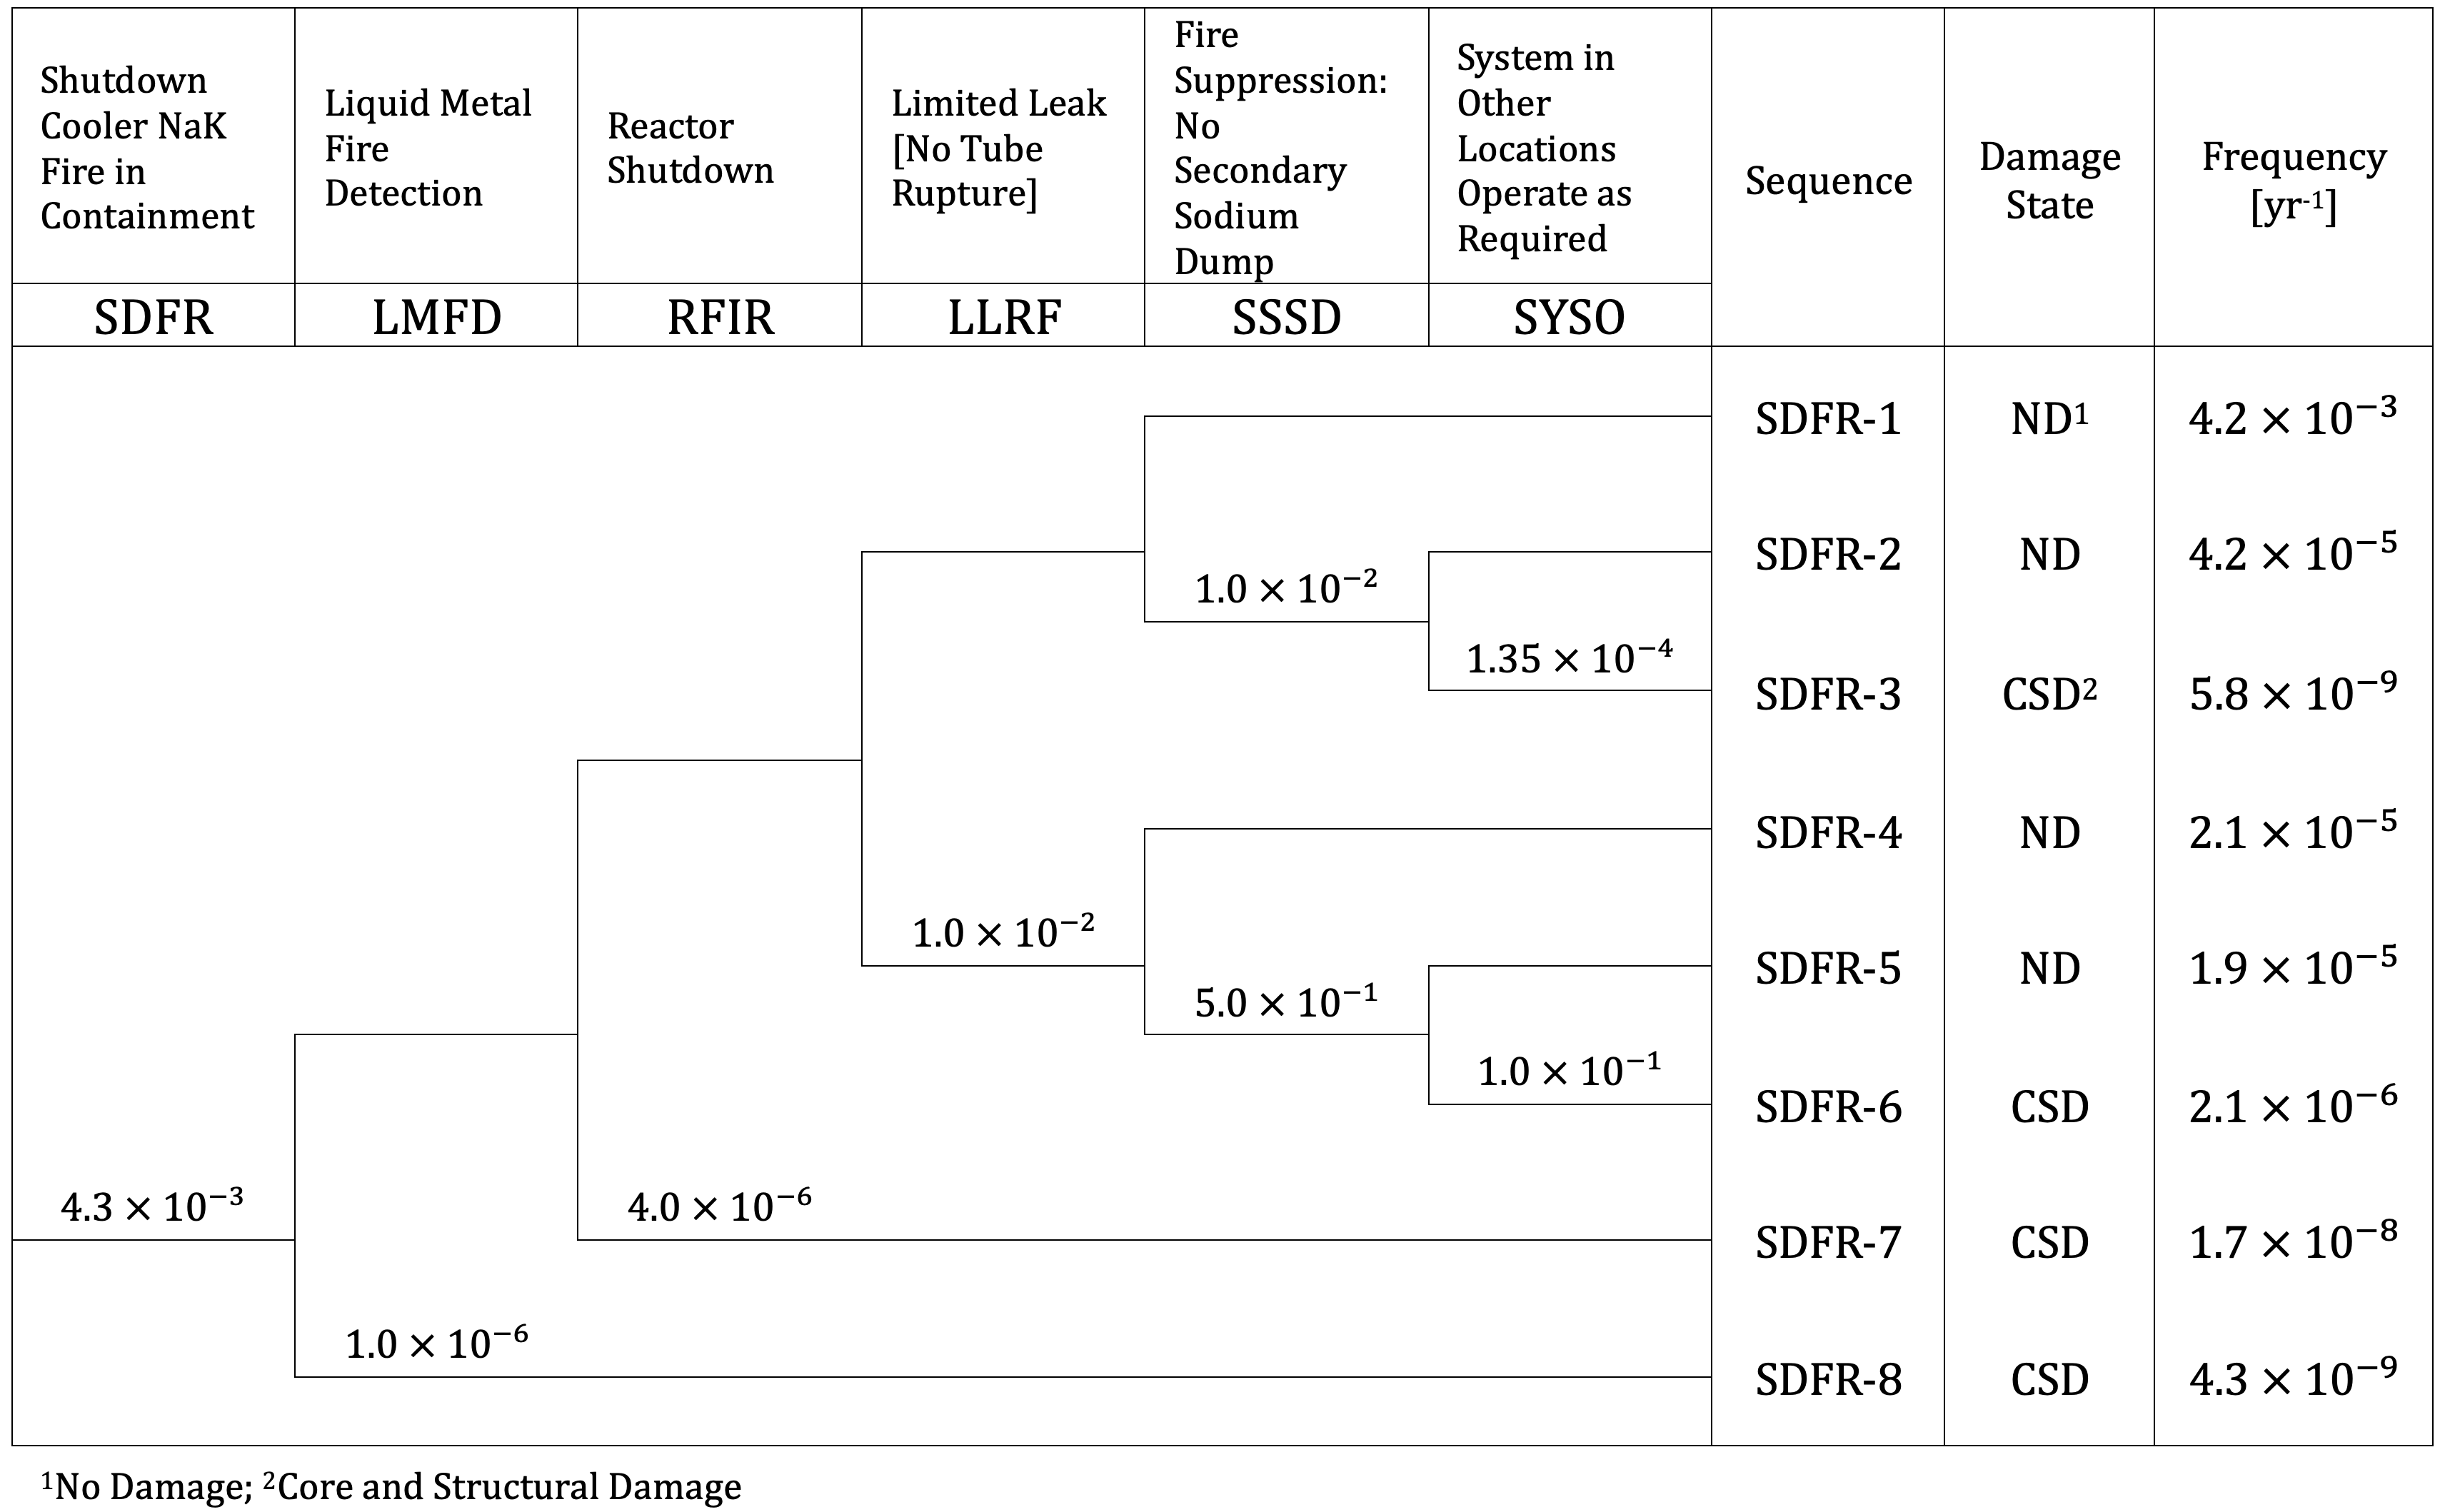
\includegraphics[width=1.0\textwidth]{parts/4_learning/1_param/figs/event_tree_NaK_fire.png} 
    \caption{EBR-II Shutdown Cooler NaK Fire in Containment}
    \label{fig:ebr2_sdfr_et}
\end{figure}

\subsection{Event Tree Structure and Problem Setup}
Following the notation from Section~\ref{sec:event_tree_definition}, each end-state \(S_j\) arises from a particular path of success/failure outcomes across the conditional events. Let \(\{X_1,\dots,X_n\}\) be the events (e.g., \(\text{LMFD}, \text{RFIR}, \dots\)), and let \(y_{ji}\in\{0,1,\text{NaN}\}\) indicate whether \(X_i\) fails, succeeds, or is not applicable for path \(S_j\). The probability of end-state \(S_j\) is
\begin{equation}
\label{eq:ebr2_es_probability}
P(S_j) 
\;=\;
\prod_{i=1}^{n} P\bigl(y_{ji}\bigr),
\end{equation}
where 
\begin{equation}
P\bigl(y_{ji}\bigr)
\;=\;
\begin{cases}
P\bigl[X_i = 1\bigr], & \text{if } y_{ji}=1,\\
1 - P\bigl[X_i = 1\bigr], & \text{if } y_{ji}=0,\\
1, & \text{if } y_{ji}=\text{NaN}.
\end{cases}
\label{eq:ebr2_conditional}
\end{equation}
Thus, one may represent each end-state \(S_j\) by multiplying the associated conditional event probabilities along its branch of the tree.

In this case study, each \(P\bigl[X_i=1\bigr]\) is assigned a (truncated) log-normal parameterization, reflecting the fact that event probabilities can span several orders of magnitude. Let \(\mu_i,\sigma_i\) denote the log-space mean and standard deviation of event \(X_i\). Under truncation rules (e.g., restricting \(\mu_i\in[10^{-10},1]\) and \(\sigma_i\in[10^{-10},10^{4}]\)), the resulting probability stays in \((0,1)\) and avoids extreme instabilities. These are plotted in Figure \ref{fig:conditionals_initial} as normalized kernel density estimates\cite{terrell_variable_1992}.

\subsection{Loss Function Definition}
Given a set of target or observed end-state frequencies \(\{p_{j}^{\mathrm{obs}}\}_{j=1}^m\), the task is to infer \(\{\mu_i,\sigma_i\}_{i=1}^n\) so that the predicted frequencies 
\[
p_{j}^{\mathrm{pred}}\;\equiv\;P\bigl(S_j \mid \{\mu_i,\sigma_i\}\bigr)
\]
match \(p_{j}^{\mathrm{obs}}\) as closely as possible. Denoting \(\boldsymbol{\theta}=(\mu_1,\sigma_1,\dots,\mu_n,\sigma_n)\) for all events, the optimal parameters solve a constrained minimization:
\begin{equation}
\label{eq:ebr2_optimization}
\min_{\boldsymbol{\theta}\in\Omega}
\quad
\mathcal{L}\bigl(\boldsymbol{\theta};\,\{p_{j}^{\mathrm{obs}}\}\bigr)
\quad
\text{subject to truncation and system constraints,}
\end{equation}
where \(\Omega\) encodes bounds (e.g., \(\mu_i,\sigma_i \ge 10^{-10}\)), and \(\mathcal{L}\) is a loss function. Here, one defines \(\mathcal{L}\) via a Normalized Relative Logarithmic Error (NRLE), which balances discrepancies in both the predicted end-state frequencies and the tails of the distributions. A simplified version of NRLE is:
\begin{equation}
\label{eq:ebr2_nrle}
\text{NRLE} 
\;=\;
\frac{1}{m}
\sum_{j=1}^{m}
\;\frac{1}{2}
\Bigl(
  \text{MAE}\bigl(\log[p_{j}^{\mathrm{obs}}+\epsilon],\,\log[p_{j}^{\mathrm{pred}}+\epsilon]\bigr)
  \;+\;
  \text{MAE}\bigl(\sigma_{j}^{\mathrm{obs}},\,\sigma_{j}^{\mathrm{pred}}\bigr)
\Bigr),
\end{equation}
where \(\text{MAE}\) denotes mean absolute error, and \(\epsilon\) is a small positive constant to avoid \(\log(\,0\,)\). The terms \(\sigma_{j}^{\mathrm{obs}}\) and \(\sigma_{j}^{\mathrm{pred}}\) refer to log-space standard deviations for the respective distributions of (or mapped from) end-states or functional events. By design, this objective penalizes deviations of both central tendencies and spread. A gradient-based algorithm (e.g., Adam \citep{zhang_improved_2018}) then iteratively refines \(\{\mu_i,\sigma_i\}\), using automatic differentiation with respect to \(\mathcal{L}\).
